\chapter{Tecnologias Utilizadas}

\section{Tecnologia de comunicação}
A partir de todo o levantamento teórico e considerando-se o contexto do problema, a tecnologia que mostrou mais destaque, foi o Bluetooth. 

Mais especificamente, a indrodução do Bluetooth Low Energy (BLE) tornou tal tecnologia bem favorável ao uso para localização, devido ao seu baixo consumo energético, mantendo caracteristicas similares de comunicação.

As principais características da escolha podem ser encontradas abaixo:\newline

\textbf{Economia e eficiência energética} \newline
Uma das principais vantagens da tecnologia Bluetooth para a localização indoor é sua alta eficiencia energética. O custo da instalação de um sistema com BLE é baixo quando em comparação de outras tecnologias já que um dispositivo equipado com um chip de BLE pode de 1 a 2 anos com uma unica bateria moeda (\textit{coin cell}).No contexto de um armazém, a economia de custos é fundamental. \newline

\textbf{Acessibilidade e Escalabilidade} \newline
Como mencionado, estima-se que até 2022 400 milhões de dispositivos de localização baseados em Bluetooth sejam vendidos por ano \cite{art9}. Fazendo-o uma tecnologia prontamente acessível e com varios recursos de desenvolvimento.

Para o contexto do projeto, uma rápida implementação é desejável. Além disso, estar presente em dispositivos atuais é um requisito, dado que deseja-se a instalação do sistema com o minimo de mudança na infraestrutura atual. Bluetooth está presente na maioria dos telefones celulares, os quais poderiam se integrar ao sistema prontamente. \newline

\textbf{Precisão}\newline
A precisão necessária é tal que dois SKUs (Unidade de Manutenção de Estoque) em localidades diferentes possam ser diferenciados. Para isso, uma precisão de até 1m é desejada.

Com a técnologia Bluetooth e os algoritmos corretos tal precisão pode ser alcançada.\newline

\textbf{Latência}\newline
A latência no Bluetooth é elevada quando comparada à outras tecnologias. Para aplicações que precisão de localização em tempo real pode ser uma desvantagem. Entretanto no projeto em questão os ativos ficam estáticos no armazém. E a latência não se torna um problema tão grande.\newline

\section{Propriedades do sinal}
Os principais algoritmos mencionados anteriormente exigem para sua implementação uma distância conhecida e um ângulo conhecido para um ponto de referência. No presente trabalho, será utilizado o RSSI para estimar a distância e o AoA para estimar o ângulo.

Quando um chip de Bluetooth recebe o sinal ele é capaz de retornar o valor da intensidade desse sinal, então a obtenção do RSSI é direta e não exige nenhum hardware adicional. Apesar de não ser o método mais preciso para estimar distância, seu custo beneficio é alto.

Já para estimar o ângulo, será utilizado o AoA. Tal propriedade em conjunto com a de intensidade do sinal permite que algoritmos estimem uma localização com uma precisão muito maior quando em comparação a algoritmos que utilizam apenas a intensidade do sinal. Assim, apesar de necessitar de um hardware mais complexo, o ganho é alto.

Nas especificações do Bluetooth anteriores à 5.1 lançada em Janeiro de 2019, a obtenção do AoA exigia um hardware extra.
Entretanto, dados os recentes avanços na tecnologia agora é possivel estimar o ângulo de chegada de um sinal se o chip Bluetooth utilizada possuir suporte para Bluetooth 5.1 ou superior.

Uma alternativa para estimar o AoA para especificações anteriores à 5.1 é a utilização de um interferômetro de 6-portas, que é um dispositivo que é baseado nas superposições deslocadas de fase das ondas incidentes e refletidas em uma porta. Diferentes defasagens de fase resultam em diferentes potências nas portas de saída da arquitetura de um 6-portas \cite{art14}.

Abaixo um desenho esquemático da arquitetura de um 6-portas: 

\begin{figure}[H]
	\centering 
	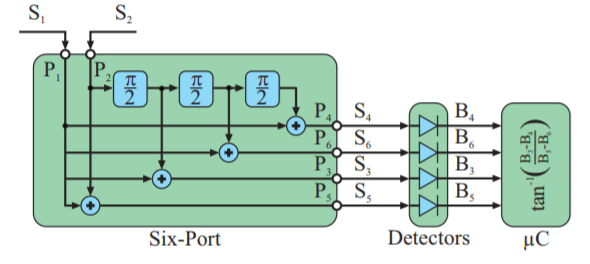
\includegraphics[scale = 1]{images/six_port_schematic.png}
	\caption{Esquemático de uma arquitetura 6-portas. Tirado de \cite{art14} }
	\label{fig:six_port_schematic}
\end{figure}

Na figura \ref{fig:six_port_schematic} os símbolos \( S_1 \) e \( S_2 \) representam os de sinais de entrada e \( S_3 \) a \( S_6 \) representam as potências medidas na saída. Já os simbolos de \( B_3 \) a \( B_6 \) representam as potências de \( S_3 \) a \( S_6 \) convertidas para tensões de base.

As equações que relacionam esses sinais são:

\begin{align*}
    S_3 & = 0.5(S_1 + jS_2) & B_3 = \left | S_3 \right | ^2\\
    S_4 & = 0.5(S_1 - jS_2) & B_4 = \left | S_4 \right | ^2\\
    S_5 & = 0.5(S_1 + S_2)  & B_5 = \left | S_5 \right | ^2\\
    S_6 & = 0.5(S_1 - S_2)  & B_6 = \left | S_6 \right | ^2
\end{align*}

A partir disso, é possível encontrar diversas propriedades úteis dos sinais incidente, tais como a a diferença de fase  \( \Delta\phi\), a distância do sinal \( \Delta\delta\) e a propriedade que mais interessa para o presente trabalho, o ângulo de chegada \(\theta\) a partir das seguintes equações:

\begin{equation}
    Z = (B_5 - B_6) + j(B_3 - B_4)
    \end{equation}

\begin{equation}
    \Delta \phi = \arctan \left ( \frac{B_3-B_4}{B_5-B_6} \right )
    \end{equation}

\begin{equation}
    \Delta d = \lambda \frac{\arg\left ({Z}  \right ) }{4\pi }
    \end{equation}

\begin{equation} \label{eq:eq_AoA}
    \theta = \sin^{-1}{(\frac{\lambda \Delta \phi}{2\pi a} )}
    \end{equation}

Em que Z é um número complexo que relaciona as tensões de saída, \(\lambda\) é o comprimento de onda do sinal e \(a\) a distância entre antenas receptoras.

A referência \cite{art15} apresenta um maior detalhamento da arquitetura. Para o contexto de localização indoor, as equações forneceriam o ângulo \(\theta\) desejado.

\section{Prova de Conceito}
Para validar o projeto final, foi proposta uma prova de conceito que aplica as tecnologias mencionadas para obter uma estimativa de distância a partir do Bluetooth.
No projeto final algoritmos, e técnicas mais elaboradas serão utilizados para uma maior precisão, porém na prova de conceito, é possível validar o projeto e mostrar os potenciais de atingir o objetivo final do projeto.

A seguir um detalhamento de como foi elaborada a prova de conceitos e os resultados atingidos.

\subsection{Hardware}
O Hardware escolhido para prova de conceito é a placa de desenvolvimento nRF52840 DK da fabricante de componentes Nordic Semiconductor \cite{nRF52840_site}.

Tal placa de desenvolvimento conta com o SoC nRF52840 que possui Bluetooth 5.0 integrado, e pinos de GPIO com entrada analógica, além de um amplo suporte de recursos online para o desenvolvimento. Soma-se a isso, sua compatibilidade com o SoC nRF52811 da mesma fabricante, que é um dos unicos chips atualmente que possui Bluetooth 5.1 e planeja-se utilizar na etapa final do projeto \cite{nRF52811_site}.

Como o nRF52840 DK não possui suporte para AoA, e placas de desenvolvimento do nRF52811 serão disponibilizadas somente no próximo semestre pela Nordic Semiconductor, pretende-se utilizar um interferômetro de 6-portas desenvolvido no departamento de sistemas eletrônicos da escola politécnica da USP para estimar o ângulo de chegada.

O interferômetro possuí 4 saídas analógicas. Fazendo-se a leitura dessas 4 saídas e utilizando a equação \ref{eq:eq_AoA} encontra-se o AoA.

\begin{figure}[H]
	\centering 
	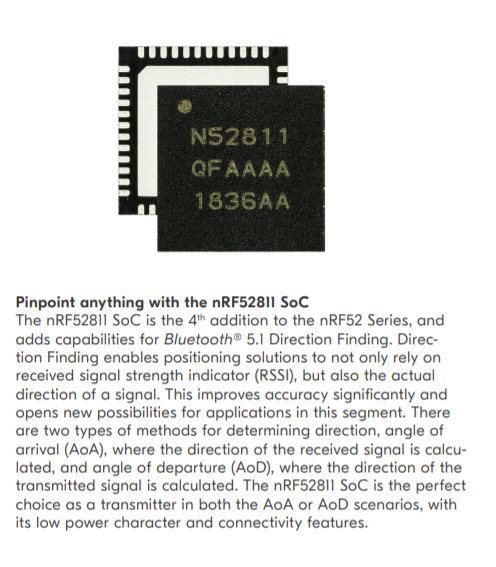
\includegraphics[scale = 1]{images/nRF52811.png}
	\caption{nRF52811. Tirado de \cite{nRF52811_site}}
	\label{fig:nRF52811}
\end{figure}


\begin{figure}[H]
	\centering 
	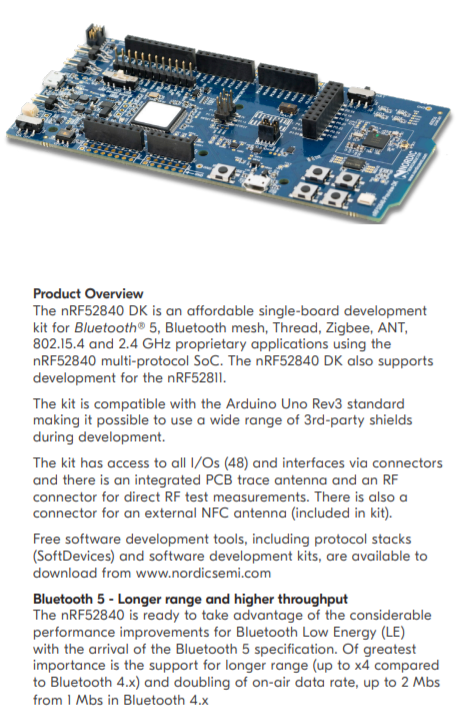
\includegraphics[scale = 1]{images/nRF52840_dk.png}
	\caption{nRF52840. Tirado de \cite{nRF52840_site}}
	\label{fig:nRF52840_dk}
\end{figure}




\subsection{Firmware}

\subsection{Arranjo Experimental}

\subsection{Resultados}


